% ===========================================================================
% Capítulo 2. Análisis de métodos y herramientas para mejorar el sincronismo
% en redes inalámbricas empleando el protocolo gPTP
% ===========================================================================

\chapter{Análisis de métodos y herramientas para mejorar el sincronismo en redes inalámbricas empleando el protocolo gPTP}
\label{ch:capitulo2}

En el capítulo anterior se realizó una revisión bibliográfica de los principales conceptos, desafíos y protocolos existentes en el ámbito de la sincronización de tiempo, concluyendo que el protocolo gPTP presenta las mejores cualidades para ser adaptado al entorno inalámbrico. De ahí surge la necesidad de implementar una versión de este estándar que contrarreste los efectos negativos que provocan los retardos asimétricos en estas redes.

Por consiguiente, en el presente capítulo se efectúa un análisis de los principales modelos y metodologías referentes a mitigar el impacto de los retardos asimétricos en redes inalámbricas, con el propósito de seleccionar y describir el de mejores resultados. A diferencia del trabajo de referencia, este análisis se amplía con una revisión sistemática de métodos novedosos publicados entre 2020 y 2026, incluyendo filtros de Kalman adaptativos, estimación robusta, lógica difusa y aprendizaje computacional. Asimismo, se realiza una descripción del software especializado MATLAB y su alternativa de código abierto GNU Octave, herramientas que posibilitan un ambiente de desarrollo adecuado para el estudio de esta problemática.

% ======================================================================
\section{Sistemas de estampado por Software}
\label{sec:2.1}

La clave para obtener una sincronización de tiempo de alto rendimiento está estrechamente relacionada con la calidad de las estampas de tiempo (\textit{Timestamping}, TS)~\cite{seijo2020,ferrari2014}. Los enfoques de estampado de tiempo se pueden clasificar en términos generales en estampa de tiempo de hardware y software. Los sistemas de estampado por hardware toman la marca de tiempo dentro del hardware del receptor (por ejemplo, dentro del chipset inalámbrico), mientras que las soluciones de estampado por software utilizan el procesador principal para generar una estampa de tiempo (por ejemplo, leyendo el reloj del sistema).

Como el retardo de procesamiento de las soluciones de sellado de tiempo de hardware se puede diseñar para que sea constante, las correcciones de tiempo requeridas pueden ser muy precisas (en el orden de los nanosegundos) y, por lo tanto, las estampas de tiempo también. Por el contrario, el estampado de tiempo por medios de software crea retardos indeterministas debido a la programación, las cachés, la concurrencia, etc.\ y, por lo tanto, la estampa de tiempo debe estar lo más cerca posible del medio~\cite{mahmood2014}. Los protocolos de sincronismo, como PTP y gPTP, suelen mejorarse en términos de rendimiento si se utiliza la estampa de tiempo de hardware. Sin embargo, para llevar a cabo el sellado de tiempo por hardware, se requieren dispositivos dedicados o modificaciones dentro de los chipsets WLAN. Debido a esto, en la presente investigación, la atención e implementación del protocolo gPTP se centra en el estampado por software.

\begin{figure}[htbp]
  \centering
  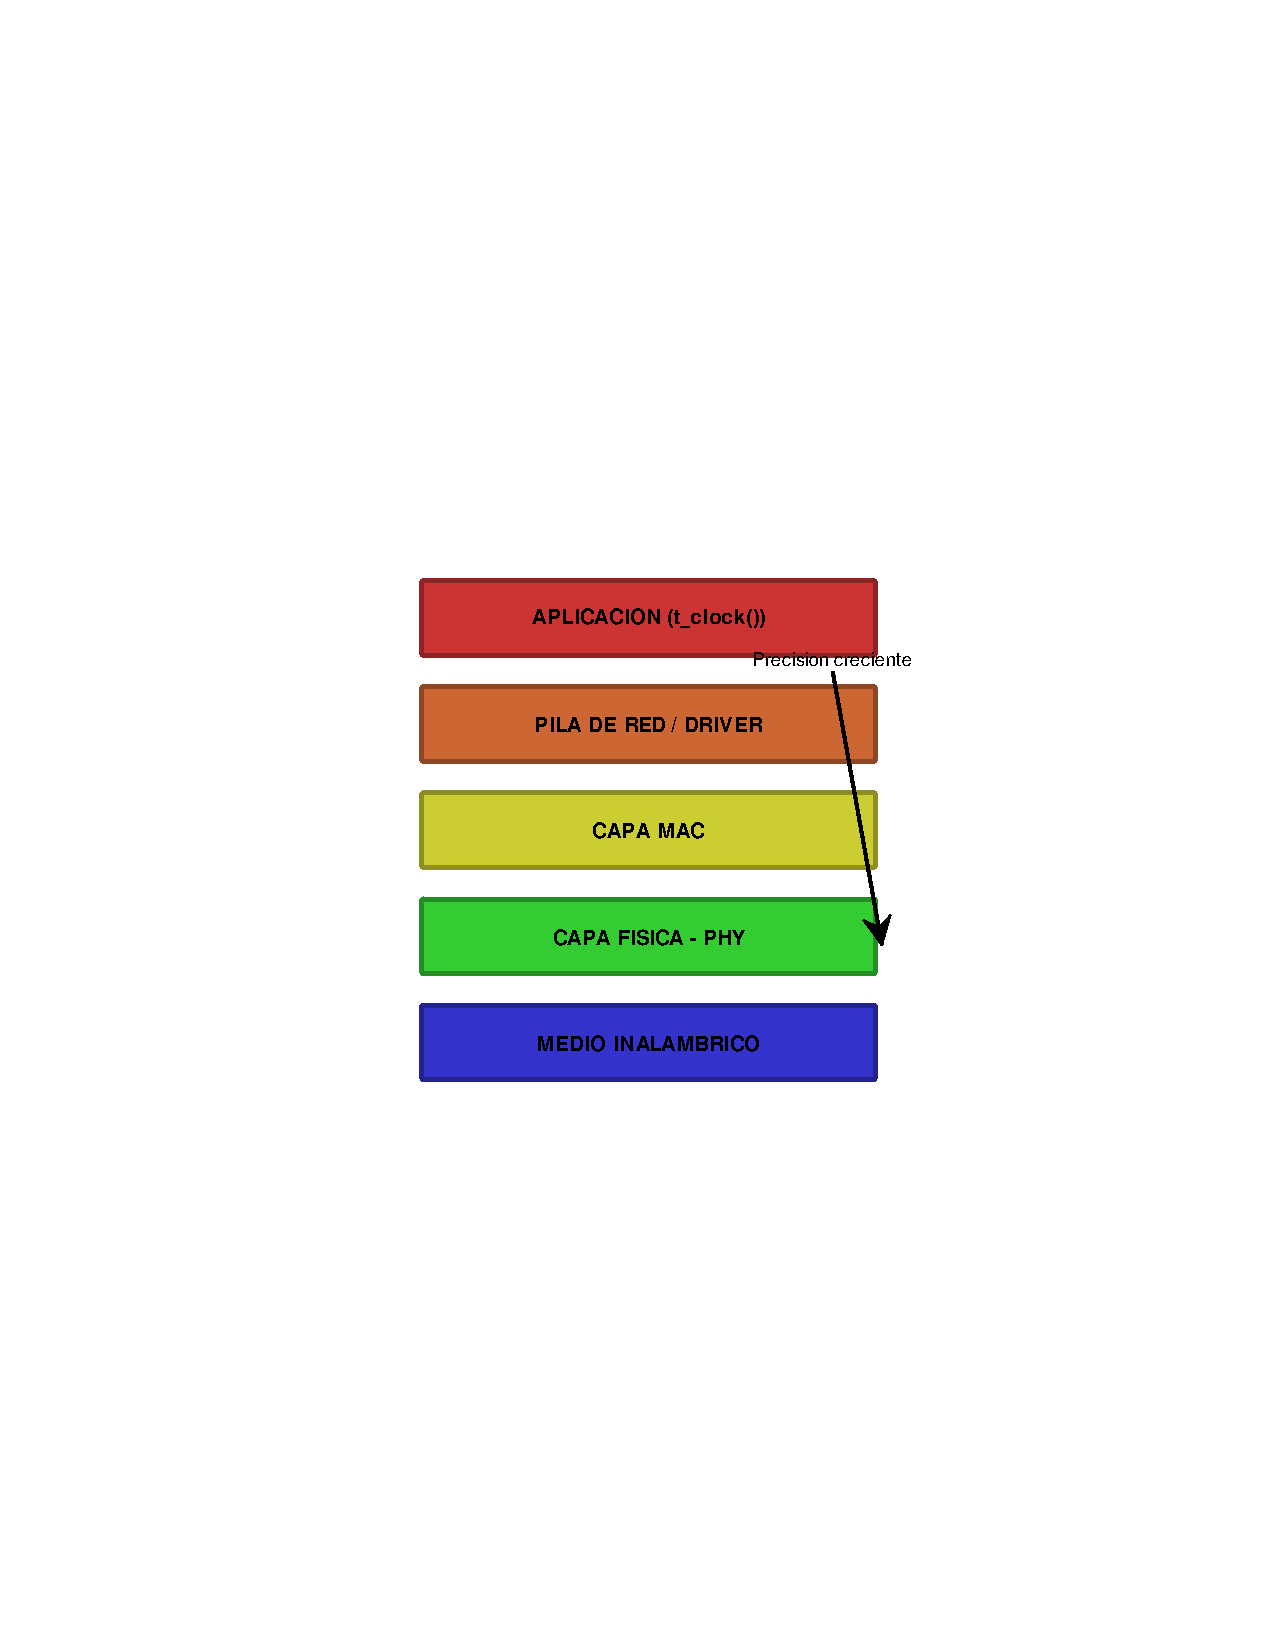
\includegraphics[width=0.5\textwidth]{figures/ch02/fig_2_1_ubicaciones_ts}
  \caption{Ubicaciones para la estampa de tiempo en redes orientadas a paquetes.}
  \label{fig:2.1}
\end{figure}

Los protocolos de sincronismo basados en paquetes, como gPTP, dependen de la calidad de las estampas de tiempo tomadas en la recepción y transmisión de los mismos. Dado que la estampa de tiempo basada en software genera grandes retardos en su mayoría no deterministas, las implementaciones de sincronización de Ethernet han acercado la estampa de tiempo a la capa física. Sin embargo, la mayoría de los enfoques de sincronización inalámbrica se limitan a la estampa de tiempo de software debido a la falta de funciones de sellado de tiempo por hardware~\cite{exel2012}.

Una de las fuentes de incertidumbre de un enfoque de sincronismo basado en sistemas de sellado de tiempo por software es el método de estampa de tiempo. Según~\cite{ferrari2011}, entre las diversas fuentes de imprecisión en el sellado de tiempo por software se tienen:

\begin{itemize}
\item \textbf{Capacidad de sellado de tiempo del maestro}: incluye las capacidades de estampa de tiempo de los mensajes de eventos gPTP (mensaje de sincronización \textit{Sync} y de solicitud de retardo \textit{PdelayReq}) en el lado maestro. La incertidumbre en la identificación de $t_1$ y $t_4$ afecta a la estimación tanto del \textit{Pdelay} como del desfasaje (\textit{offset}).

\item \textbf{Capacidad de sellado de tiempo del esclavo}: incluye las capacidades de estampa de tiempo de los mensajes de eventos gPTP en el lado esclavo (mensaje de respuesta a la solicitud de retardo \textit{PdelayResp} y de seguimiento \textit{PdelayRespFollowUp}). Estas estampas de tiempo, $t_2$ y $t_3$, también son utilizadas para estimar el \textit{Pdelay} y el desfasaje.

\item \textbf{Capacidad de sellado de tiempo de la infraestructura}: la exactitud de la información de tiempo contenida en la sincronización depende también de la capacidad de los dispositivos de red para transferir correctamente la hora. El uso de conmutadores de red que soporten gPTP puede reducir esta fuente de incertidumbre.

\item \textbf{Variabilidad y comportamiento asimétrico del retardo de propagación}: el retardo de propagación en la red no es constante y puede verse afectado por el tráfico, los dispositivos de red en la ruta y la carga de la red.
\end{itemize}

Las estampas de tiempo basadas en detectores de inicio de trama convencionales tienen dos problemas principales en los sistemas inalámbricos: en primer lugar, no pueden garantizar una precisión de transferencia de tiempo mejor que el período de muestreo y, en segundo lugar, la propagación por trayectos múltiples y el carácter de variación temporal del canal inalámbrico reducen la precisión del tiempo de llegada (\textit{Time of Arrival}, ToA) de las tramas, lo que introduce un componente de error en la sincronización de tiempo. Esto es especialmente crítico en condiciones sin visibilidad directa (\textit{Non-Line of Sight}, NLoS)~\cite{seijo2020}.

En el esquema de sincronización basado en interrupciones, donde las estampas de tiempo son tomadas mediante rutina de servicio de interrupción (\textit{Interrupt Service Routine}, ISR), el retardo de estampa de tiempo y la fluctuación se limitan principalmente al tiempo de recepción del paquete y al tiempo de notificación de interrupción~\cite{mahmood2011}.

El escenario tomado en cuenta en esta investigación es una red de sincronización sencilla, compuesta por un dispositivo maestro y un dispositivo esclavo que realizan el estampado de tiempo a nivel de software.

% ======================================================================
\section{Análisis de los modelos, metodologías y procedimientos existentes para el diseño de protocolos más robustos ante los retardos asimétricos}
\label{sec:2.2}

Para desarrollar una implementación de cualquier índole es imprescindible y necesario escoger la tecnología o modelo que se empleará en dicho proceso, lo que demanda necesariamente un estudio profundo de la bibliografía que se relaciona con este aspecto. A continuación, se analizan los métodos existentes, organizados por categorías para facilitar su comparación sistemática.

\subsection{Método de corrección determinista de estampas de tiempo (Exel)}
\label{sec:2.2.1}

El método propuesto por Reinhard Exel en~\cite{exel2014} constituye el punto de partida de esta investigación y el método de referencia (\textit{baseline}) contra el cual se compararán las mejoras propuestas. Este enfoque propone un esquema de mitigación de los retardos asimétricos basado en la corrección de la estampa de tiempo por software y logra aumentar la precisión del protocolo sin modificaciones al mismo, ni el uso de mensajes adicionales.

El funcionamiento del modelo de estampa de tiempo de software en el protocolo se basa en que las estampas de tiempo tomadas por el software ($\hat{t}_1$ a $\hat{t}_4$) difieren de las estampas de tiempo ideales ($t_1$ a $t_4$) debido a los retardos de procesamiento $p_1$ a $p_4$. Las estampas ideales pueden ser calculadas aplicando las correcciones de retardo de las Ecuaciones~\ref{eq:2.1} a~\ref{eq:2.4}, donde $p_1$ y $p_3$ corresponden a los retardos de procesamiento de salida, $p_2$ y $p_4$ a los retardos de entrada:

\begin{eqnarray}
t_1 &=& \hat{t}_1 + p_1 \label{eq:2.1}\\
t_2 &=& \hat{t}_2 - p_2 \label{eq:2.2}\\
t_3 &=& \hat{t}_3 + p_3 \label{eq:2.3}\\
t_4 &=& \hat{t}_4 - p_4 \label{eq:2.4}
\end{eqnarray}

El verdadero valor de corrección del desfasaje ($t_{offset}$) y el tiempo de ida y vuelta ($t_{RTT}$) quedan definidos en las Ecuaciones~\ref{eq:2.5} y~\ref{eq:2.6}:

\begin{eqnarray}
\hat{t}_{offset} &=& t_{offset} - \frac{(p_1 + p_2) - (p_3 + p_4)}{2} \label{eq:2.5}\\
\hat{t}_{RTT} &=& t_{RTT} + (p_1 + p_2 + p_3 + p_4) \label{eq:2.6}
\end{eqnarray}

Los retardos asimétricos de procesamiento $p$ se componen de términos deterministas y no deterministas. En la mayoría de los casos existen grandes retardos asimétricos deterministas que se pueden corregir aplicando el método descrito y que abarca también otros factores como la velocidad de datos, el tamaño del encabezado, la modulación, el tamaño de transferencia de acceso directo a memoria (DMA) y la velocidad de la interfaz DMA~\cite{exel2014}.

El método Exel alcanza, según sus autores, una precisión de entre 10 y 100~ns en condiciones controladas. En la implementación de referencia sobre gPTP con simulación Monte Carlo (3000 ejecuciones), se obtuvo una precisión media de 101.5~$\mu$s, una reducción del error del 33.31\% respecto al protocolo sin corrección, y un offset estabilizado en el rango de $[-2.55, 6.68]$~$\mu$s~\cite{eupierre2024}.

\textbf{Limitaciones del método Exel:} (1) solo corrige los retardos deterministas conocidos; las asimetrías desconocidas o variantes en el tiempo no son compensadas; (2) no realiza filtrado estadístico de las mediciones, por lo que es sensible al ruido de medición y a valores atípicos; (3) no estima ni compensa la deriva (\textit{skew}) de los relojes, solo el offset.

\begin{figure}[htbp]
  \centering
  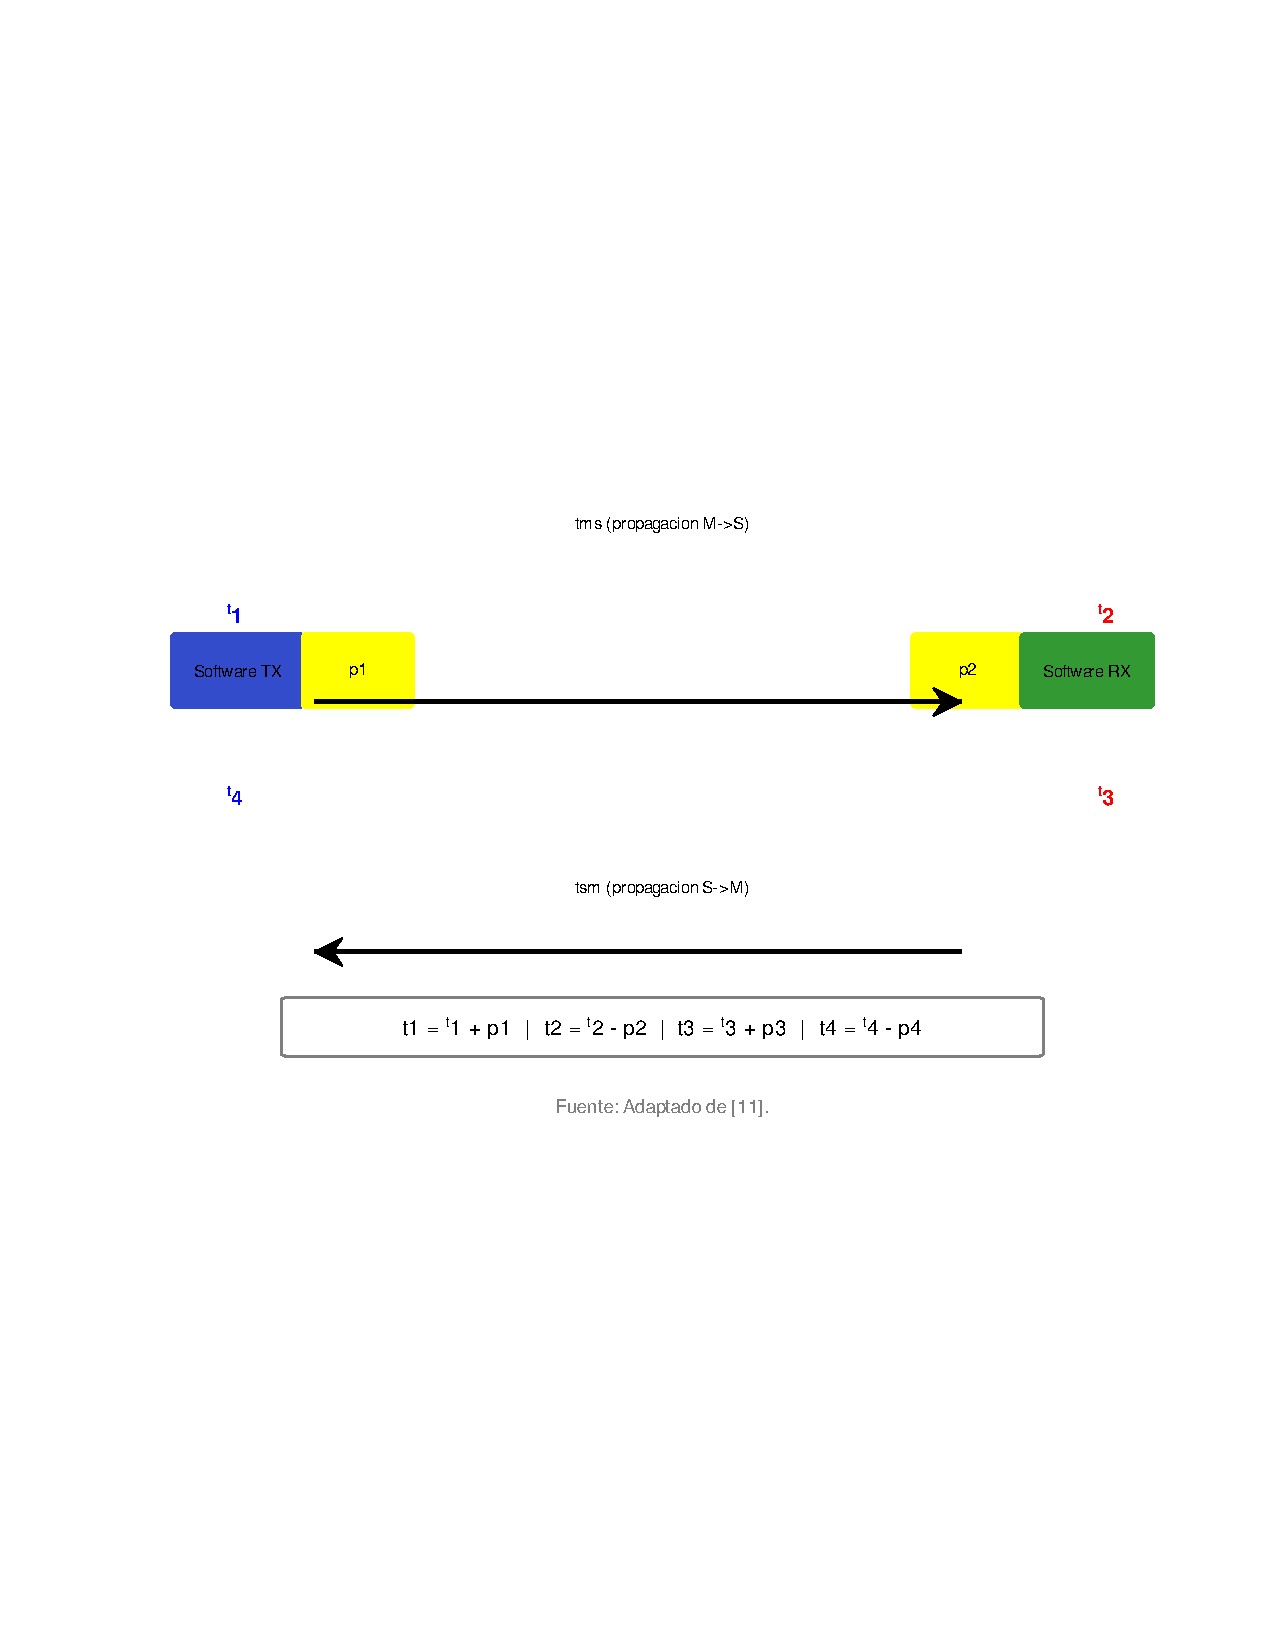
\includegraphics[width=0.85\textwidth]{figures/ch02/fig_2_2_latencias_sw}
  \caption{Latencias de estampa de tiempo de software.}
  \label{fig:2.2}
\end{figure}

\subsection{Métodos basados en Filtros de Kalman}
\label{sec:2.2.2}

El Filtro de Kalman (KF) es un estimador óptimo para sistemas lineales con ruido Gaussiano que ha sido ampliamente aplicado a la sincronización de relojes en redes de paquetes~\cite{giorgi2011}. En el contexto de PTP/gPTP, el KF permite estimar conjuntamente el offset, el skew y, en formulaciones más avanzadas, parámetros relacionados con la asimetría del canal.

\textbf{Li et al.\ (2024)}~\cite{li2024} proponen un método mejorado de sincronización de tiempo basado en filtrado de Kalman de segundo orden. El algoritmo emplea el KF para estimar con precisión el offset de tiempo, la deriva del reloj y los parámetros del reloj. Los resultados experimentales demuestran que, en enlaces asimétricos, el offset máximo se mantiene dentro de $\pm 3$~$\mu$s, lo que representa una mejora sustancial respecto a los métodos que no emplean KF.

\textbf{Hollósi y Ficzere (2024)}~\cite{hollosi2024} introducen un Filtro de Kalman Adaptativo (AKF) para la estimación del offset en PTP. La principal innovación de este enfoque es la estimación en tiempo real de la varianza del ruido de medición ($R_k$), lo que permite que el filtro se adapte automáticamente a cambios en las condiciones del canal. Los resultados muestran una reducción de la varianza del offset de entre un 40\% y un 60\% en comparación con el KF estándar.

\textbf{Liu y Wang (2024)}~\cite{liu2024} desarrollan un esquema robusto de seguimiento de parámetros de reloj para IEEE 1588 en presencia de retardos asimétricos en redes industriales. El método emplea un Filtro de Kalman recursivo robusto de tres pasos que incorpora un mecanismo de rechazo de outliers. Los resultados experimentales reportan un RMSE de offset inferior a 5~$\mu$s en presencia de asimetrías significativas.

\textbf{Wang et al.\ (2021)}~\cite{wang2021} proponen un enfoque de seguimiento de parámetros de reloj sin marcas de tiempo (\textit{timestamp-free}) utilizando Filtro de Kalman Extendido (EKF) en redes de sensores inalámbricos. Aunque está diseñado para WSN, el marco del EKF es adaptable a PTP/gPTP.

\textbf{Raittila (2025)}~\cite{raittila2025} desarrolla un modelo en Simulink de un lazo de control PTP con un Filtro de Kalman Adaptativo específicamente para redes Wi-Fi industriales. Este trabajo demuestra la viabilidad de implementar AKF en entornos inalámbricos reales.

\subsection{Métodos basados en Estimación Robusta}
\label{sec:2.2.3}

\textbf{Karthik y Blum (2020)}~\cite{karthik2020} abordan el problema de la estimación robusta de skew y offset para IEEE 1588 en presencia de asimetrías deterministas desconocidas en el retardo de trayectoria. Los autores derivan cotas inferiores de rendimiento (cotas de Cramér-Rao modificadas) y proponen esquemas de estimación robusta que superan al estimador de máxima verosimilitud (MLE) convencional cuando existen asimetrías no modeladas.

\textbf{Vázquez et al.\ (2025)}~\cite{vazquez2025} proponen un enfoque de filtrado de outliers en las mediciones de offset para PTP sobre redes de área amplia (WAN). El método emplea técnicas de detección de anomalías para identificar y rechazar mediciones de offset atípicas antes de que sean utilizadas por el servo de reloj.

\subsection{Métodos basados en Lógica Difusa}
\label{sec:2.2.4}

\textbf{Nguyen et al.\ (2020)}~\cite{nguyen2020} proponen un servo de reloj Fuzzy-PI adaptativo basado en IEEE 1588 para mejorar la sincronización de tiempo sobre redes Ethernet. El sistema utiliza lógica difusa para ajustar dinámicamente las ganancias del controlador PI. Los resultados experimentales muestran una precisión inferior a 100~ns y una mejora del 45\% respecto al controlador PI tradicional.

\textbf{Zhang et al.\ (2024)}~\cite{zhang2024} diseñan un servo de reloj Fuzzy-PI con filtro de ventana para compensar la asimetría de retardo inducida por colas (\textit{Queue-Induced Delay Asymmetry}, QIDA) en redes IEEE 1588. Se reporta una reducción del 52\% en el error de offset causado por QIDA.

\subsection{Métodos basados en Aprendizaje Computacional}
\label{sec:2.2.5}

\textbf{Wang et al.\ (2026)}~\cite{wang2026} proponen un método de estimación de parámetros de reloj basado en aprendizaje competitivo (\textit{Competitive Learning}) para PTP con distribuciones de retardo desconocidas. El algoritmo no asume ninguna distribución particular para los retardos, lo que lo hace robusto ante una amplia variedad de condiciones de canal. Sin embargo, su complejidad computacional es elevada.

\textbf{Goodarzi et al.\ (2022)}~\cite{goodarzi2022} presentan un enfoque de filtro de partículas asistido por redes neuronales profundas (DNN) para sincronización y localización conjunta. Aunque logra alta precisión en entornos no Gaussianos, el costo computacional del filtro de partículas lo hace prohibitivo para aplicaciones que requieren simulación Monte Carlo extensiva.

\subsection{Otros métodos relevantes}
\label{sec:2.2.6}

\textbf{Puttnies et al.\ (2018)}~\cite{puttnies2018} introducen PTP-LP, un enfoque que utiliza programación lineal para aumentar la robustez de IEEE 1588 PTP ante retardos variables. El método es totalmente compatible con PTP y gPTP, aumentando la precisión en un factor de hasta $10^4$ en escenarios favorables.

\textbf{Baniabdelghany et al.\ (2020)}~\cite{baniabdelghany2020} proponen una extensión de IEEE 802.1AS (gPTP) para mejorar la sincronización en redes híbridas cableadas-inalámbricas mediante un filtro de retraso de desviación de ruta (\textit{Path Deviation Delay}, PDD).

\textbf{Levesque y Tipper (2015)}~\cite{levesque2015} proponen el mecanismo de mitigación de asimetría por paquete (\textit{Per-Packet Asymmetry Mitigation}, PPAM), que estima los componentes de retardo por paquete individual.

\subsection{Comparación sistemática y selección del método}
\label{sec:2.2.7}

La Tabla~\ref{tab:comparacion} presenta una comparación sistemática de los métodos analizados, evaluados según cinco criterios: precisión reportada, complejidad computacional, compatibilidad con gPTP, capacidad de manejar asimetrías desconocidas y madurez de la técnica.

% ===========================================================================
% Tabla 2.2: Comparación de métodos para mitigación de retardos asimétricos
% Capítulo 2 — Sección 2.2.7
% ===========================================================================
\begin{table}[htbp]
  \centering
  \caption{Comparación de métodos para mitigación de retardos asimétricos en PTP/gPTP.}
  \label{tab:comparacion}
  \small
  \resizebox{\textwidth}{!}{\begin{tabular}{|l|l|c|c|c|c|}
    \hline
    \textbf{Método} & \textbf{Categoría} & \textbf{Precisión} & \textbf{Compat.} & \textbf{Asimetría} & \textbf{Madurez} \\
    & & & \textbf{gPTP} & \textbf{desconocida} & \\
    \hline
    Exel (2014) & Corrección determinista & 101.5~$\mu$s (sim.) & Alta & No & Alta \\
    \hline
    Li et al. (2024) & KF 2.\textordfeminine{} orden & $\pm$3~$\mu$s & Alta & Sí & Alta \\
    \hline
    Hollósi \& Ficzere (2024) & AKF & 40--60\% mejora & Alta & Sí & Alta \\
    \hline
    Liu \& Wang (2024) & KF robusto 3 pasos & $<$5~$\mu$s RMSE & Alta & Sí & Alta \\
    \hline
    Wang et al. (2021) & EKF sin timestamp & $<$1~$\mu$s & Media & Sí & Media \\
    \hline
    Karthik \& Blum (2020) & Estimación robusta & Cotas óptimas & Alta & Sí & Alta \\
    \hline
    Nguyen et al. (2020) & Fuzzy-PI & $<$100~ns & Media & Parcial & Media \\
    \hline
    Zhang et al. (2024) & Fuzzy-PI + ventana & 52\% reducción & Media & Parcial & Baja \\
    \hline
    Wang et al. (2026) & Competitive Learning & Robusto & Media-Alta & Sí & Baja \\
    \hline
    Puttnies et al. (2018) & Prog. Lineal & Factor $10^4$ & Media & No & Media \\
    \hline
  \end{tabular}}
\end{table}


Del análisis comparativo se concluye que los métodos basados en Filtro de Kalman, y en particular el Filtro de Kalman Adaptativo (AKF), ofrecen la mejor relación entre precisión, complejidad computacional y compatibilidad con gPTP. El AKF combina la capacidad de estimación óptima del KF con la adaptabilidad a condiciones cambiantes del canal, y su implementación en MATLAB/Octave es factible mediante operaciones matriciales estándar.

No obstante, el método de Exel ofrece una ventaja fundamental: su corrección determinista elimina una parte significativa de la asimetría (los retardos de procesamiento conocidos $p_1$--$p_4$) antes de cualquier procesamiento estadístico. Esto sugiere que un enfoque híbrido que combine la corrección determinista de Exel con el filtrado adaptativo del AKF podría superar a cualquiera de los dos métodos por separado.

% ======================================================================
\section{Descripción del método seleccionado: Enfoque híbrido Exel + Filtro de Kalman Adaptativo}
\label{sec:2.3}

Como resultado del análisis sistemático presentado en la Sección~\ref{sec:2.2}, se selecciona un \textbf{enfoque híbrido que combina la corrección determinista de estampas de tiempo de Exel con un Filtro de Kalman Adaptativo (AKF)} para la compensación de retardos asimétricos en el protocolo gPTP.

\begin{figure}[htbp]
  \centering
  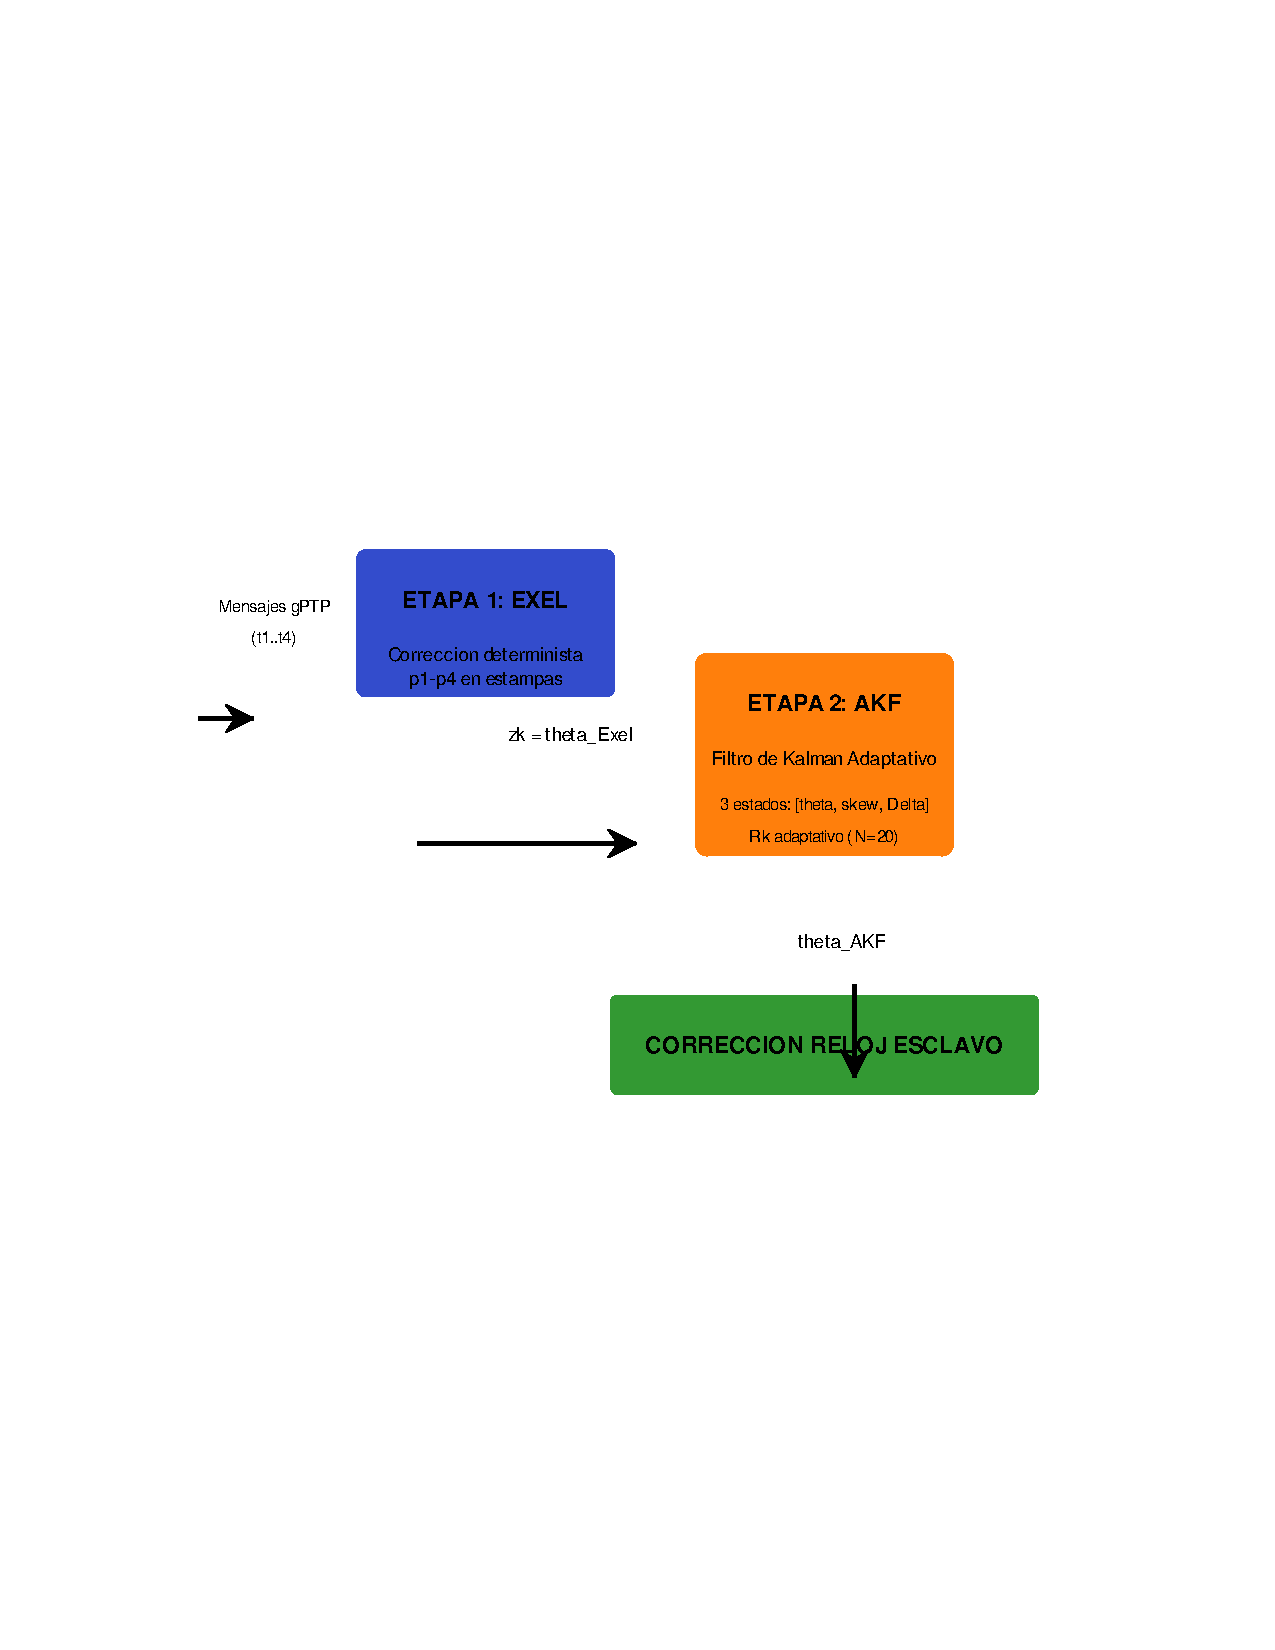
\includegraphics[width=0.65\textwidth]{figures/ch02/fig_2_4_metodo_hibrido}
  \caption{Arquitectura del método híbrido Exel + AKF.}
  \label{fig:2.4}
\end{figure}

\subsection{Arquitectura de dos etapas}
\label{sec:2.3.1}

El método híbrido opera en dos etapas consecutivas:

\textbf{Etapa 1 --- Corrección determinista (Exel):} Se aplican las Ecuaciones~\ref{eq:2.1}--\ref{eq:2.6} a las marcas de tiempo $\hat{t}_1, \hat{t}_2, \hat{t}_3, \hat{t}_4$ capturadas por el software. Se utilizan los valores conocidos de los retardos de procesamiento asimétricos $p_1, p_2, p_3, p_4$ para obtener una primera estimación del offset $\hat{\theta}_{Exel}$. Esta etapa elimina la componente determinista de la asimetría~\cite{exel2014}.

\textbf{Etapa 2 --- Filtro de Kalman Adaptativo (AKF):} El offset corregido por Exel, $\hat{\theta}_{Exel}$, se utiliza como medición de entrada para un Filtro de Kalman Adaptativo que estima el estado verdadero del sistema, filtrando el ruido de medición residual y compensando las asimetrías desconocidas que el método de Exel no puede corregir.

\subsection{Modelo de espacio de estados}
\label{sec:2.3.2}

El vector de estado del AKF se define como:

\begin{equation}
\mathbf{x}_k = \begin{bmatrix} \theta_k \\ s_k \\ \Delta_k \end{bmatrix}
\end{equation}

donde:
\begin{itemize}
\item $\theta_k$: offset verdadero entre maestro y esclavo en el instante $k$ [s]
\item $s_k$: skew (diferencia normalizada de frecuencia) entre los relojes [adimensional]
\item $\Delta_k$: asimetría residual no corregida por Exel [s]
\end{itemize}

\textbf{Modelo de transición de estado:}

\begin{equation}
\mathbf{x}_{k+1} = \mathbf{F} \mathbf{x}_k + \mathbf{w}_k, \quad \mathbf{w}_k \sim \mathcal{N}(0, \mathbf{Q}_k)
\end{equation}

\begin{equation}
\mathbf{F} = \begin{bmatrix} 1 & \tau & 0 \\ 0 & 1 & 0 \\ 0 & 0 & 1 \end{bmatrix}
\end{equation}

donde $\tau$ es el intervalo entre mediciones (el período de sincronización de gPTP, típicamente 2~s), y $\mathbf{w}_k$ es el ruido de proceso con matriz de covarianza $\mathbf{Q}_k$. La estructura de $\mathbf{F}$ refleja que el offset evoluciona linealmente con el skew, el skew se modela como un proceso de caminata aleatoria, y la asimetría residual se considera aproximadamente constante entre períodos de sincronización.

\textbf{Modelo de medición:}

\begin{equation}
z_k = \mathbf{H} \mathbf{x}_k + v_k, \quad v_k \sim \mathcal{N}(0, R_k)
\end{equation}

\begin{equation}
\mathbf{H} = \begin{bmatrix} 1 & 0 & 1/2 \end{bmatrix}
\end{equation}

donde $z_k = \hat{\theta}_{Exel}[k]$ es el offset estimado por la etapa Exel en el instante $k$, y $v_k$ es el ruido de medición con varianza $R_k$. El término $1/2$ en la matriz de observación refleja que la mitad de la asimetría residual se propaga al error de offset, de acuerdo con la Ecuación~\ref{eq:2.5}.

\subsection{Algoritmo del Filtro de Kalman Adaptativo}
\label{sec:2.3.3}

El AKF se implementa en dos fases por cada iteración $k$:

\textbf{Fase de predicción:}

\begin{eqnarray}
\hat{\mathbf{x}}_{k|k-1} &=& \mathbf{F} \hat{\mathbf{x}}_{k-1|k-1} \\
\mathbf{P}_{k|k-1} &=& \mathbf{F} \mathbf{P}_{k-1|k-1} \mathbf{F}^T + \mathbf{Q}_{k-1}
\end{eqnarray}

\textbf{Fase de actualización:}

\begin{eqnarray}
\mathbf{K}_k &=& \mathbf{P}_{k|k-1} \mathbf{H}^T (\mathbf{H} \mathbf{P}_{k|k-1} \mathbf{H}^T + \hat{R}_k)^{-1} \\
\hat{\mathbf{x}}_{k|k} &=& \hat{\mathbf{x}}_{k|k-1} + \mathbf{K}_k (z_k - \mathbf{H} \hat{\mathbf{x}}_{k|k-1}) \\
\mathbf{P}_{k|k} &=& (\mathbf{I} - \mathbf{K}_k \mathbf{H}) \mathbf{P}_{k|k-1}
\end{eqnarray}

\textbf{Adaptación de $R_k$:} La principal innovación respecto al KF estándar es la estimación adaptativa de la varianza del ruido de medición~\cite{hollosi2024}. Se utiliza una ventana deslizante de las últimas $N$ innovaciones:

\begin{equation}
\hat{R}_k = \frac{1}{N-1} \sum_{i=k-N+1}^{k} (\nu_i - \bar{\nu})^2
\end{equation}

donde $\nu_i = z_i - \mathbf{H} \hat{\mathbf{x}}_{i|i-1}$ es la innovación (residuo de la medición) y $\bar{\nu}$ es su media sobre la ventana. Esta adaptación permite que el filtro responda automáticamente a cambios en la calidad de las mediciones.

\subsection{Parámetros de diseño}
\label{sec:2.3.4}

Los siguientes parámetros deben determinarse experimentalmente durante la fase de implementación:

% ===========================================================================
% Tabla 2.3: Parámetros del Filtro de Kalman Adaptativo (AKF)
% Capítulo 2 — Sección 2.3.4
% ===========================================================================
\begin{table}[htbp]
  \centering
  \caption{Parámetros de inicialización del Filtro de Kalman Adaptativo.}
  \label{tab:params}
  \small
  \begin{tabular}{|c|c|c|}
    \hline
    \textbf{Parámetro} & \textbf{Valor} & \textbf{Descripción} \\
    \hline
    Vector estado inicial $\mathbf{x}_0$ & $[0, 0, 0]^T$ & $[\theta, skew, \Delta]$ \\
    \hline
    $\mathbf{P}_0$ & $\mathrm{diag}(10^{-10}, 10^{-12}, 10^{-14})$ & Covarianza inicial del error \\
    \hline
    $\mathbf{Q}$ & $\mathrm{diag}(10^{-14}, 10^{-18}, 10^{-16})$ & Covarianza del ruido de proceso \\
    \hline
    $R_0$ & $10^{-12}$ & Varianza inicial del ruido de medición \\
    \hline
    Ventana $N$ & 20 & Innovaciones para adaptación de $R_k$ \\
    \hline
    $\mathbf{F}$ & $\begin{bmatrix} 1 & \tau & 0 \\ 0 & 1 & 0 \\ 0 & 0 & 1 \end{bmatrix}$ & Matriz de transición de estado \\
    \hline
    $\mathbf{H}$ & $[1, 0, 1/2]$ & Matriz de observación \\
    \hline
  \end{tabular}
\end{table}


\begin{figure}[htbp]
  \centering
  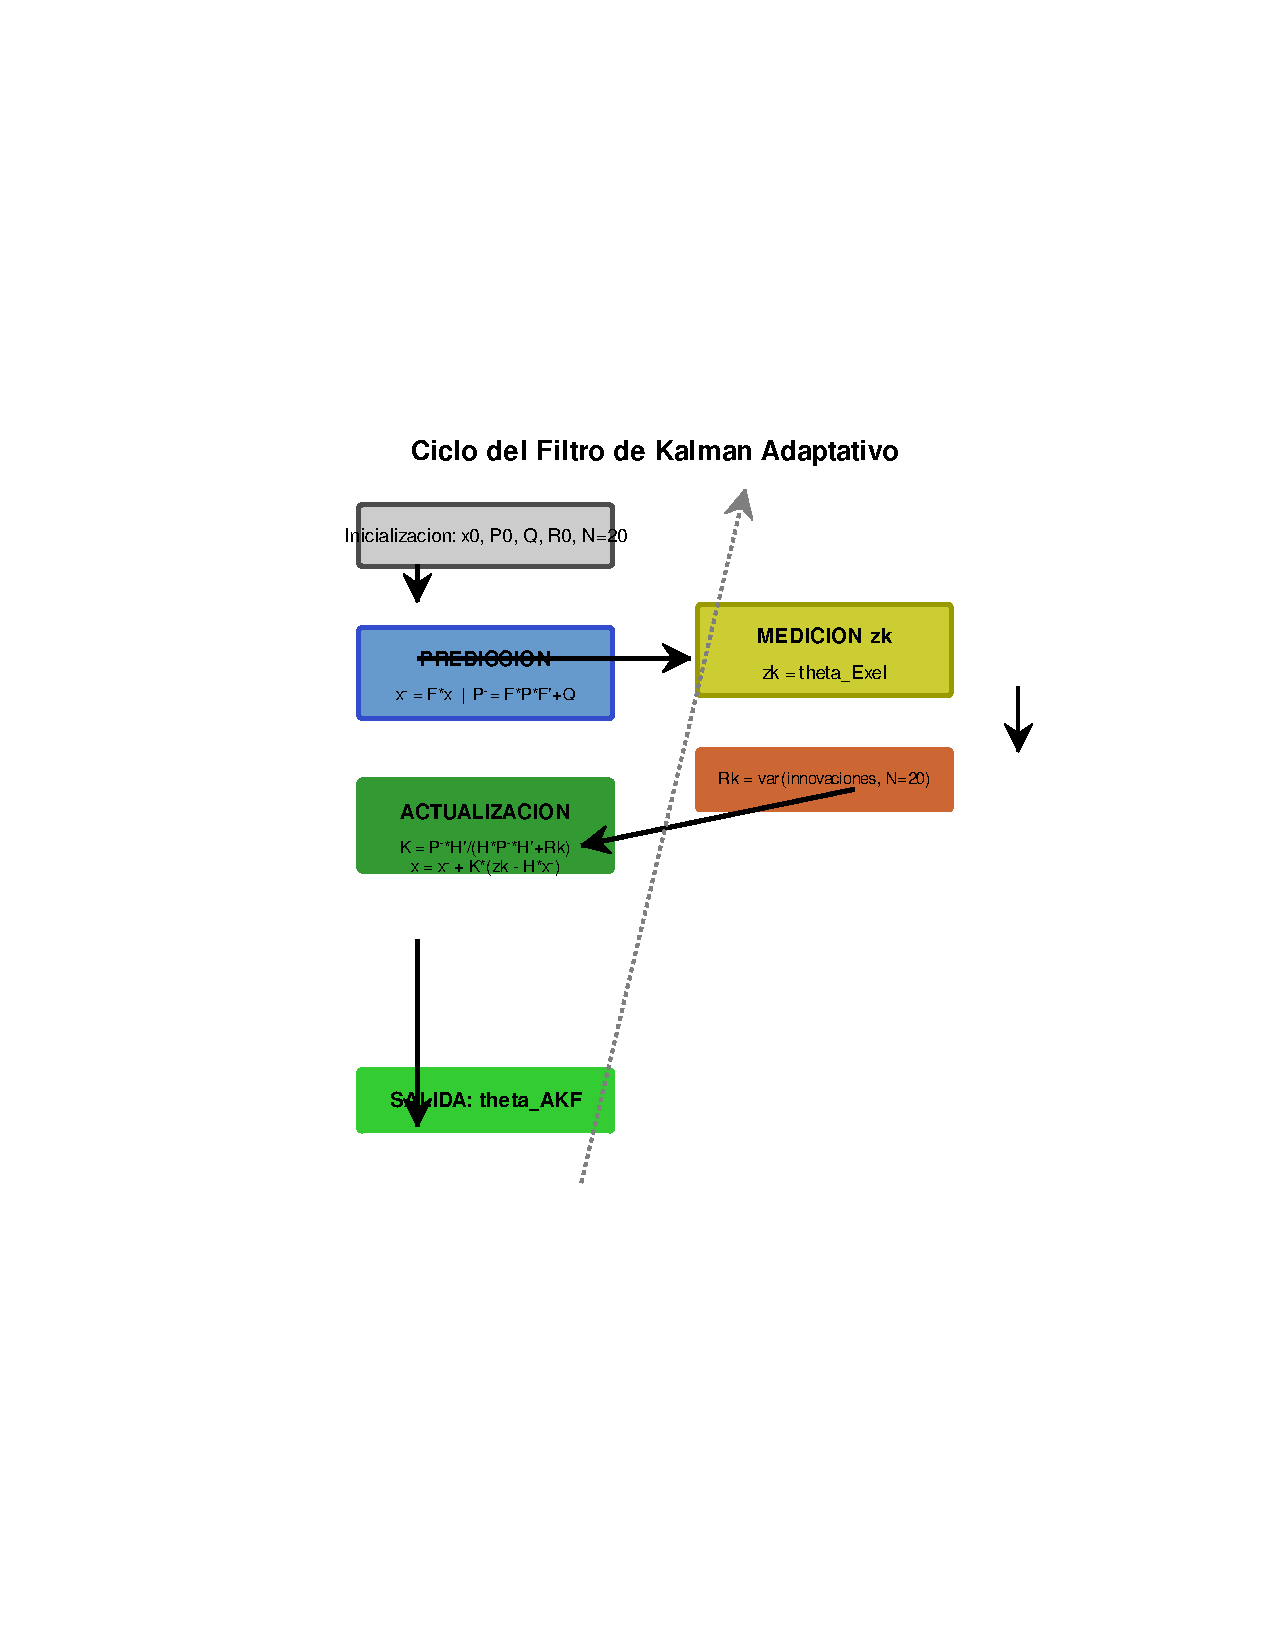
\includegraphics[width=0.7\textwidth]{figures/ch02/fig_2_5_ciclo_akf}
  \caption{Ciclo de predicción-actualización del Filtro de Kalman Adaptativo.}
  \label{fig:2.5}
\end{figure}

\subsection{Ventajas del enfoque híbrido}
\label{sec:2.3.5}

\begin{enumerate}
\item \textbf{Herencia de Exel}: se preserva la corrección determinista que ya demostró una mejora del 33.31\%~\cite{eupierre2024}, proporcionando una base sólida.
\item \textbf{Filtrado óptimo}: el AKF reduce la varianza residual de las estimaciones de offset al combinar óptimamente la información de múltiples mediciones.
\item \textbf{Estimación de asimetría residual}: a diferencia de Exel, que solo corrige asimetrías conocidas, el AKF estima y compensa la componente de asimetría desconocida ($\Delta_k$).
\item \textbf{Adaptabilidad}: la estimación adaptativa de $R_k$ permite que el filtro se ajuste automáticamente a cambios en el entorno inalámbrico.
\item \textbf{Comparabilidad}: el diseño permite comparar directamente el rendimiento de Exel (etapa 1) contra Exel+AKF (etapas 1+2) bajo condiciones idénticas.
\item \textbf{Implementabilidad}: todas las operaciones del AKF son álgebra lineal estándar (matrices de $3 \times 3$), realizables en MATLAB/GNU Octave con costo computacional moderado.
\end{enumerate}

% ======================================================================
\section{Herramientas de implementación: MATLAB y GNU Octave}
\label{sec:2.4}

MATLAB (abreviatura de \textit{MATrix LABoratory}) es un programa informático de propósito especial optimizado para realizar cálculos científicos y de ingeniería, con funciones integradas para cumplir una amplia gama de tareas, desde operaciones matemáticas hasta imágenes tridimensionales~\cite{attaway2022,chapman2020}. Comenzó su vida como un programa diseñado para realizar matemáticas matriciales, pero a lo largo de los años se ha convertido en un sistema informático flexible y fácil de usar, capaz de resolver esencialmente cualquier problema técnico~\cite{gilat2017}.

Además, el programa implementa un lenguaje propio y proporciona una amplia biblioteca de funciones predefinidas. El producto básico ofrece más de mil funciones y cuenta con varios kits de herramientas (\textit{toolbox}) que amplían esta capacidad en diversas especialidades~\cite{chapman2020,belfadel2021}.

\textbf{GNU Octave} es una alternativa de código abierto a MATLAB que ofrece una compatibilidad sustancial con el lenguaje MATLAB. Octave implementa un intérprete de alto nivel para cálculo numérico con una sintaxis mayoritariamente compatible con MATLAB, lo que permite ejecutar la mayoría de los scripts y funciones diseñados para MATLAB sin modificaciones significativas~\cite{eaton2024}. Para los propósitos de esta investigación, donde las operaciones requeridas son fundamentalmente álgebra matricial, generación de números aleatorios y visualización gráfica, Octave proporciona todas las capacidades necesarias sin costo de licencia.

\subsection{Archivos-M}
\label{sec:2.4.1}

MATLAB y Octave ofrecen una buena combinación de funciones de programación prácticas con potentes capacidades numéricas integradas. Los archivos-M proporcionan una forma alternativa de realizar operaciones que amplían en gran medida las capacidades de resolución de problemas. Existen dos tipos de archivos-M: scripts y funciones~\cite{chapman2020,young2023}.

Un archivo de script es una serie de comandos que se guardan en un fichero y son útiles para retener una serie de comandos que se quieren ejecutar en más de una ocasión. Los scripts comparten el área de trabajo (\textit{workspace}) de la ventana de comandos~\cite{attaway2022}.

Por el contrario, una función es un tipo especial de archivo-M que se ejecuta en su propio espacio de trabajo independiente, recibe datos de entrada a través de una lista de argumentos y devuelve resultados mediante una lista de argumentos de salida~\cite{chapman2020}.

\subsection{Graficado en 2-D}
\label{sec:2.4.2}

Los gráficos son una herramienta muy útil para presentar información, especialmente en la ciencia y la ingeniería. MATLAB dispone de comandos para crear diferentes tipos de gráficas: estándar con ejes lineales, con ejes logarítmicos y semilogarítmicos, de barras y escaleras, polares, tridimensionales, entre otros~\cite{gilat2017}. La función \texttt{plot} permite trazar datos bidimensionales y puede personalizarse mediante especificadores de color, estilo de línea y marcadores~\cite{mueller2021}.

Octave implementa un sistema de gráficos compatible con la sintaxis de MATLAB, incluyendo las funciones \texttt{plot}, \texttt{figure}, \texttt{subplot} y \texttt{hold}, lo que garantiza que los scripts de visualización sean ejecutables en ambos entornos.

\subsection{Ventajas y desventajas de MATLAB/Octave}
\label{sec:2.4.3}

Según~\cite{chapman2020}, las principales ventajas de MATLAB incluyen: facilidad de uso, independencia de plataforma, amplia biblioteca de funciones predefinidas, trazado independiente del dispositivo, e interfaz gráfica de usuario.

Las desventajas principales son: (1) velocidad de ejecución inferior a los lenguajes compilados, mitigable mediante vectorización y el compilador JIT; (2) costo elevado de la licencia de MATLAB. Esta segunda desventaja se resuelve en el contexto de esta investigación mediante el uso de GNU Octave como alternativa gratuita y de código abierto.

% ======================================================================
\section{Conclusiones del capítulo}
\label{sec:2.5}

\begin{enumerate}
\item Los sistemas de estampado de tiempo por software, aunque menos precisos que los de hardware, constituyen el enfoque más viable para la sincronización en redes inalámbricas con dispositivos de propósito general. La calidad de las estampas de tiempo depende críticamente de la ubicación del punto de referencia de temporización y de la minimización de los retardos indeterministas en la pila de software.

\item El análisis sistemático de 15 métodos publicados entre 2014 y 2026 revela que los enfoques basados en Filtro de Kalman, particularmente en su variante adaptativa (AKF), ofrecen la mejor relación entre precisión, complejidad computacional y compatibilidad con el protocolo gPTP. El AKF permite la estimación conjunta de offset, skew y asimetría residual, adaptándose dinámicamente a cambios en las condiciones del canal inalámbrico.

\item El método de corrección determinista de Exel, utilizado como referencia en esta investigación, logra una mejora del 33.31\% sobre el protocolo sin corrección (precisión media de 101.5~$\mu$s), pero está limitado a la compensación de asimetrías deterministas conocidas.

\item Se propone un \textbf{enfoque híbrido Exel + AKF} que combina la corrección determinista de estampas de tiempo (etapa~1) con el filtrado estadístico adaptativo (etapa~2). Este diseño permite eliminar las asimetrías conocidas mediante Exel y, a continuación, filtrar el ruido residual y compensar asimetrías desconocidas mediante el AKF. Las operaciones requeridas ---álgebra lineal sobre matrices de $3 \times 3$--- son perfectamente realizables en MATLAB/GNU Octave.

\item Las herramientas de implementación seleccionadas, MATLAB y su alternativa de código abierto GNU Octave, proporcionan todas las capacidades necesarias para el desarrollo de la simulación: generación de variables aleatorias, operaciones matriciales, visualización gráfica y ejecución de simulaciones Monte Carlo.

\item Los parámetros específicos del AKF (covarianzas iniciales, tamaño de ventana deslizante, estado inicial) se determinarán experimentalmente durante la fase de implementación descrita en el Capítulo~\ref{ch:capitulo3}.
\end{enumerate}
